\subsection{Description of Product / Structure: Describe the creative ideation and what is new?}

Our product is a Mars capable ATV. We began with the idea of the standard ATV, coupled with the idea of a manned Mars rover. By combining these two concepts, we were able to create a more agile vehicle capable of handling Mars’ low gravity and dusty environment. The combination of a pressurized capsule in an off-road vehicle can be challenging but the benefits would be immense in creating robust vehicles for a manned colony on Mars.

\subsection{Description of subsystem}

\begin{center}
\begin{tabular}{lll}
\hline
Subsystem & Description\\
\hline
Orbital Deployment & Circular parachute and coiled spring shocks.\\
Grabbers & Pivoting arm with ball socket and grabbing hands.\\
Suspension & Coil spring shocks, double A-frame suspension and tire rods.\\
Chassis & Triangular truss support frame. \\
Tires & Cylindrical tires with embossed treads. \\
Controls & Joystick,Displays, Plexiglas encased w/ rectangular control panel.\\
Cockpit & Oblong shaped cockpit \\
Powertrain & Circular Motor with chain drive to rear axle with rear diff.\\
Charging & Rectangular solar cells on roof. \\
Science/Storage & Large prismed storage area in back of ATV. \\
Communication System & Conic Satellite Dish. \\
Lighting & Semi-Paraboloid lights mounted on front of ATV. \\
\hline
\end{tabular}
\end{center}

\subsection{Subassembly Functionality}
\begin{center}
\begin{tabular}{lll}
\hline
Subsystem & Functionality\\
\hline
Orbital Deployment & Landing Gear when ATV is dropped from orbit. \\
Grabbers & Grabs materials for data inspection.\\
Suspension & Absorbs shocks from planetary terrain. \\
Chassis & Beefy frame for surviving rough conditions.\\
Tires & Extreme grip to handle unexpected terrain. \\
Controls & Steering, cockpit, seating, etc.\\
Cockpit & Location of Controls\\
Powertrain & Electric drivetrain, differential. \\
Charging & Solar cells from roof to charge batteries behind cockpit. \\
Science/Storage & Large storage area in back of ATV to collect data/samples. \\
Communication System & Antenna to communicate with base. \\
Lighting & To maintain visibility once night falls or in sandstorms.\\
\hline
\end{tabular}
\end{center}

\subsection{Allocation for each member}

\begin{center}
\begin{tabular}{lll}
\hline
Subsystem & Member& Complexity\\
\hline
Orbital Deployment & Vishakh Kumar& Medium\\
Grabbers & Justin Sackett & Hard\\
Suspension & Asimm Hirani & Medium\\
Chassis & Juan Rodriguez & Hard\\
Tires & Auston Ferrarer& Easy\\
Controls & Vishakh Kumar & Hard\\
Cockpit & Vishakh Kumar & Easy\\
Powertrain & Asimm Hirani & Hard\\
Charging & Vishakh Kumar & Easy \\
Science/Storage & Auston Ferrarer & Medium\\
Communication System & Juan Rodriguez & Medium\\
Lighting & Justin Sackett& Easy\\
\hline
\end{tabular}
\end{center}

\subsection{Briefly explain what new functionalities (system and sub-system ) you are planning to add. How your product is different from existing products:}

This design differs from the traditional ATV because it has a improved suspension system for travel along Martian terrain. The ATV will be able to withstand orbital entry into the Martian landscape through its improved suspension and parachute for controlled descent. Additionally for increased driver visibility the pressurized cabin is built with GT-Superglass® which has the material strength of hardened steel and the weight of titanium. With this glass our vehicle will be able to withstand sandstorms containing heavy debris.

\subsection{Picture of  the Proposed System (or Similar System): (please include a reference if you are using pictures from internet). You can also include conceptual sketch.}
\begin{center}
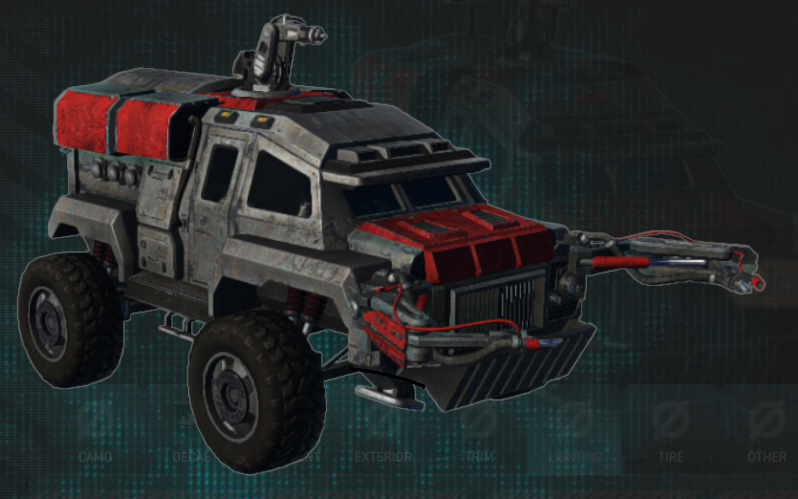
\includegraphics[width=0.75\textwidth]{a-1-1-ProjectIdeation/b-1-ProjectProposal/c-1-Images/Planetside.png} \\
(Daybreak Games: Planetside 2 ANT Vehicle Concept)

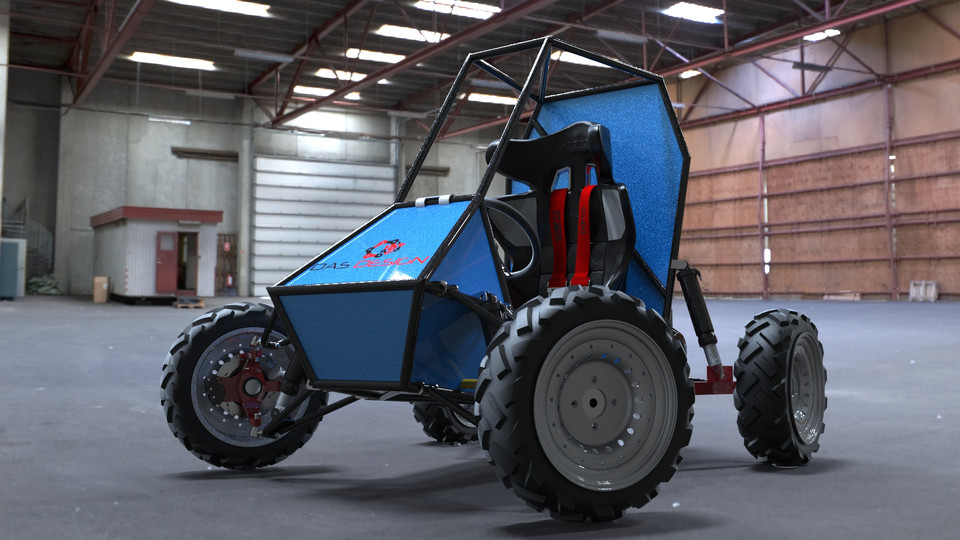
\includegraphics[width=0.75\textwidth]{a-1-1-ProjectIdeation/b-1-ProjectProposal/c-1-Images/BAJA.jpeg} \\
(https://grabcad.com/library/baja-atv-1 - BAJA SAE India Team)
\end{center}
